%!TEX root = pfc-memoria.tex
%!TEX encoding = UTF-8 Unicode

\chapter{Aprendizaje automático}

El \textbf{aprendizaje automático}\index{aprendizaje automático} (en inglés, \emph{machine learning}\index{machine learning@\emph{machine learning}}) es la rama de la Inteligencia Artificial cuyo objetivo es desarrollar técnicas que permitan a las computadoras \textbf{aprender}. De forma más concreta, se trata de crear programas capaces de generalizar comportamientos a partir de una información suministrada en forma de ejemplos de la que debe extraer el conocimiento necesario para que el programa pueda realizar automáticamente la tarea que se le pretende \citep[Aprendizaje automático]{wikipedia-es}.

Estas posibles tareas pueden ser: \citep{MartinMateos2013} 
\begin{itemize}
\item Toma de decisiones
\item Clasificación de documentos
\item Búsqueda de documentos relevantes
\item Comprensión del lenguaje
\item Recuperación de la información
\item Extracción de la información
\item Generación de discurso
\item Traducción automática
\item \ldots
\end{itemize}

\section{Concepto}

Vamos a explicar el concepto de método de aprendizaje automático para tareas de clasificación de documentos.
Formalizando el \nombrebf{problema de clasificación}\index{clasificación!problema de}, tenemos la descripción $d\in \mathbb{X}$ de un documento, dónde $\mathbb{X}$ es el espacio de documentos; y un conjunto finito de clases $\mathbb{C} = \{c_1, c_2, \ldots, c_J\}$. Estas clases también se llaman categorías o etiquetas \citep{Manning2008}.

$\mathbb{X}$ suele ser un espacio vectorial con un gran número de dimensiones, mientras que las clases son las necesarias para la aplicación. En el caso de detección de la polaridad del sentimiento, podría ser $\mathbb{C}=\{-2,-1,0,-1,-2\}$, representando a opiniones muy negativas, negativas, neutras, positivas y muy positivas.

En lugar de tener que programar manualmente cómo relacionar documentos y clases para construir el clasificador, tomaremos un conjunto de entrenamiento $\mathbb{D}$ de documentos $d$ manualmente etiquetados con su clase $\langle d, c \rangle \in \mathbb{X} \times \mathbb{C}$.

Usando un método de \nombrebf{aprendizaje automático}\index{aprendizaje automático} $\Gamma$ aplicado al conjunto de entrenamiento $\Gamma(\mathbb{D})$ obtenemos como resultado el clasificador $\gamma : \mathbb{X} \mapsto \mathbb{C}$ \citep{Manning2008} que predice la clase a la que pertenecen documentos no vistos en la fase de entrenamiento.

\section{Métodos de aprendizaje automático}

Existen básicamente dos grupos de métodos de aprendizaje automático:
\nopagebreak
\begin{description}
\item[Aprendizaje supervisado]\index{aprendizaje!supervisado} Estos algoritmos producen una función entrenada con un conjunto de entrenamiento que proporciona la entrada y también la salida (la \emph{clase}, en el caso del problema de clasificación) que se desea para el sistema.
\item[Aprendizaje no supervisado]\index{aprendizaje!no supervisado} Éstos, por el contrario, se entrenan simplemente con las entradas (en el caso de clasificación: sin necesidad de estar la muestra etiquetada con su clase).
\item[Aprendizaje semi-supervisado]\index{aprendizaje!semi-supervisado} Combina ambos tipos de aprendizaje.
\end{description}

A modo de muestra, enumeramos algunos de los algoritmos para cada tipo:
\nopagebreak
\begin{itemize}
\item Supervisados:
\begin{itemize}
\item Árboles de decisión
\item Vecinos más cercanos
\item Aprendizaje por refuerzo con retroalimentación (ensayo-error)
\item Máquinas de Vectores de Soporte (\emph{Support Vector Machines}, SVM\index{SVM})
\item Aprendizaje estadístico Naïve-Bayes
\item Redes Neuronales Artificiales
\end{itemize}
\item No supervisados:
\begin{itemize}
\item Agrupamiento plano: \emph{flat partitional clustering}
\item Agrupamiento jerárquico: \emph{hierarchical clustering}
\end{itemize}
\end{itemize}

En las figuras \ref{fig:hier-clustering} y \ref{fig:k-medias} se puede ver las diferencias en las etapas de clustering para el método de particionado plano y el jerárquico.

\begin{figure}[htbp]
\centering
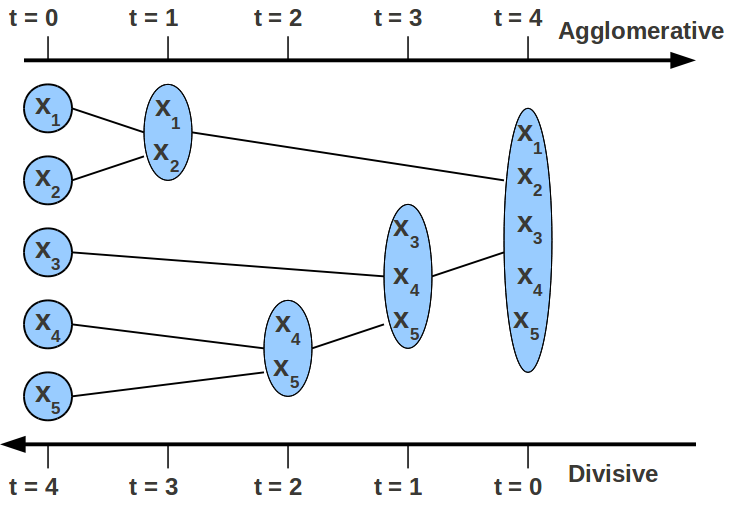
\includegraphics[width=0.6\textwidth]{hierarchical-clustering}
\caption[Etapas del agrupamiento jerárquico]{Etapas del agrupamiento jerárquico \citep{Rai2011}}
\label{fig:hier-clustering}
\end{figure}

\begin{figure}[htbp]
\centering
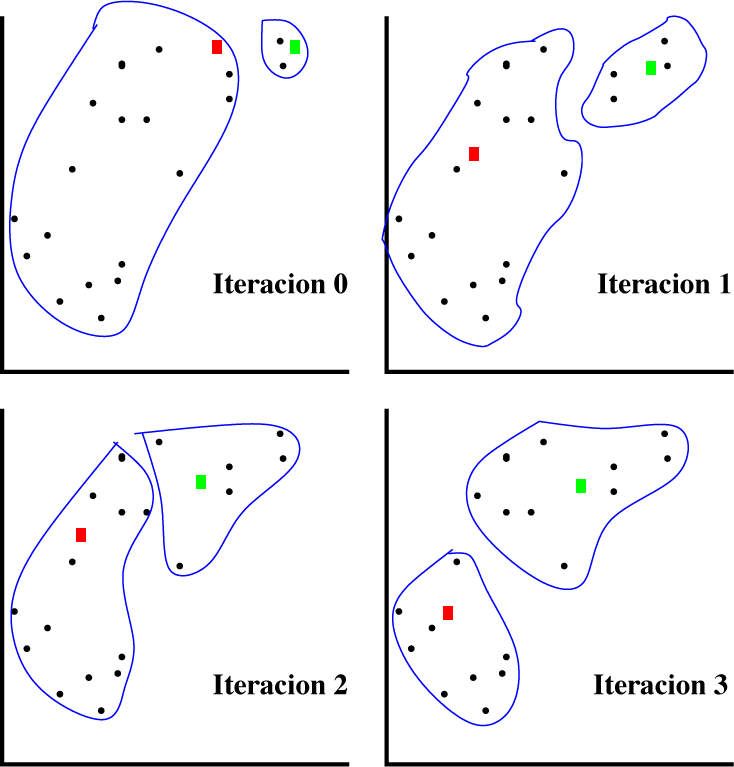
\includegraphics[width=0.6\textwidth]{k-medias}
\caption[Etapas del agrupamiento plano]{Etapas del agrupamiento plano \citep{RuizReina2013}}
\label{fig:k-medias}
\end{figure}

Además, uno de los retos de estos sistemas es cómo representar el conocimiento extraído en el entrenamiento para almacenarlo y usarlo posteriormente.

\section{Extracción de características}

En los métodos de aprendizaje que vemos en esta sección, por regla general hay que establecer un vector que represente a cada documento (frase). Todos los vectores deberán tener la misma dimensión, y cada dimensión del espacio vectorial de documentos recibe el nombre de \nombrebf{característica}\index{característica} \emph{(feature)}\index{feature@\emph{feature}}. De esta manera, un documento se equipara a un vector de valores numéricos (números en coma flotante, bien en cualquier rango o bien normalizado y acotado en el intervalo $[0,1]$); lo que se puede representar mediante un \emph{punto} dentro del espacio vectorial (\autoref{fig:feat-space}).

\begin{figure}[htbp]
\centering
\todo{pendiente dibujar mejor}
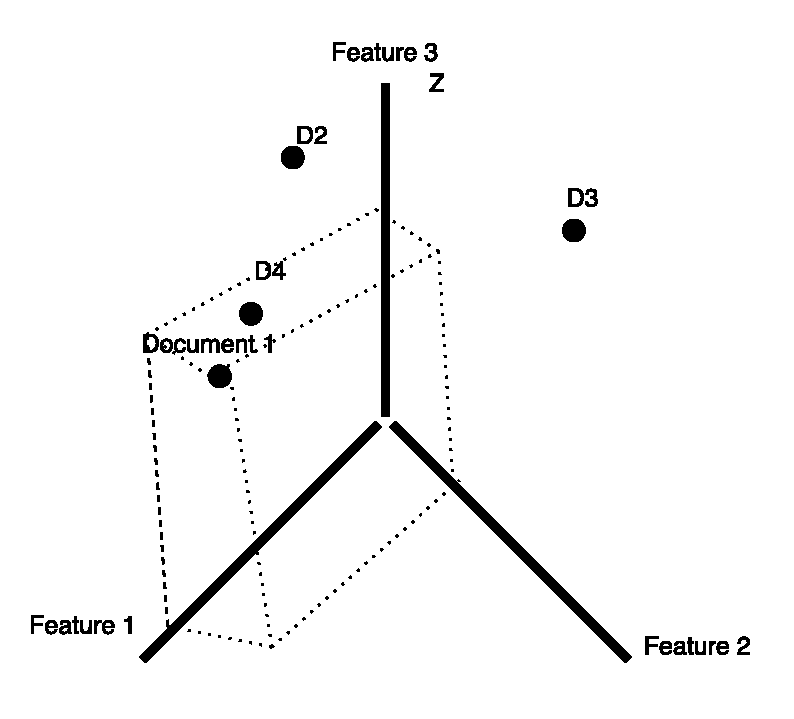
\includegraphics[width=0.6\textwidth]{feat-space}
\caption{Espacio vectorial de las características de los documentos \emph{(feature document space)}}
\label{fig:feat-space}
\end{figure}

Una vez transformado el corpus de texto de entrenamiento en un conjunto de puntos dentro del espacio vectorial, se pasa como entrada al método de aprendizaje automático. Si estos puntos llevan asociada la clase, será un aprendizaje supervisado. En caso contrario, será un aprendizaje no supervisado.

Antes de proceder al extracción de las características del texto del documento, es útil aplicar algún procesamiento como los explicados en la \autoref{sec:preproc-NLP}, ``\nameref{sec:preproc-NLP}''.

\subsection{Saco de palabras \emph{(bag-of-words)}}

\begin{definition}[saco de palabras]
Se denomina \nombrebf{saco de palabras}\index{saco de palabras} (BOW, por sus siglas en inglés de \emph{bag-of-words})\index{bag-of-words@\emph{bag-of-words}} al conjunto de palabras existente en un documento.
\end{definition}

A este saco, se le pueden eliminar las palabras vacías (stopwords) ---si es que no se le ha aplicado antes---, y además no tener en cuenta las palabras (términos) con poca frecuencia de distribución dentro del conjunto de corpus si éste es muy grande, como manera de reducir el vocabulario y mejorar el rendimiento o reducir el \nombrebf{sobreajuste}\index{sobreajuste} \emph{(overfitting)}\index{overfitting@\emph{overfitting}} del modelo.

\begin{definition}[vocabulario]
El \nombrebf{vocabulario}\index{vocabulario} es el conjunto formado por los términos que se toman en consideración para una aplicación de NLP. Se puede contemplar el uso del vocabulario común del idioma, también llamado \nombrebf{lexicón}\index{lexicón}, diccionario o tesauro\index{tesauro}.
\end{definition}

Una vez calculado el vocabulario, se usa cada término como característica, y o bien se indica con un valor 0 ó 1 si el término está presente en el documento o no, o bien el conteo del número de las apariciones del término en el mismo.

\begin{example}[Vocabulario y representación usando BOW]\label{exa:ml-bow}
Dado el siguiente conjunto de documentos:
\begin{enumerate}
\item ``A series of escapades demonstrating the adage that what is good for the goose''
\item ``demonstrating the adage that what is good for the goose''
\item ``amuses but none of which amounts to much of a story''
\end{enumerate}
Obtener el vocabulario de características y vector de representación BOW para cada documento.
\end{example}

La solución al ejercicio la calculamos con en el \autoref{lst:vocab-feat-BOW}.

\begin{listing}[htbp]
\begin{minted}{python}
>>> doc1 = "A series of escapades demonstrating the adage that what is good for the goose".split(' ')
>>> doc2 = "demonstrating the adage that what is good for the goose".split(' ')
>>> doc3 = "amuses but none of which amounts to much of a story".split(' ')
>>> features = list(set(doc1 + doc2 + doc3))
>>> features.sort()
>>> vec1 = [doc1.count(feat) for feat in features]
>>> vec2 = [doc2.count(feat) for feat in features]
>>> vec3 = [doc3.count(feat) for feat in features]
>>> print(features) # vocabulario de características
['A', 'a', 'adage', 'amounts', 'amuses', 'but', 'demonstrating', 'escapades', 'for', 'good', 'goose', 'is', 'much', 'none', 'of', 'series', 'story', 'that', 'the', 'to', 'what', 'which']
>>> print(vec1) # vector de representación del documento 1
[1, 0, 1, 0, 0, 0, 1, 1, 1, 1, 1, 1, 0, 0, 1, 1, 0, 1, 2, 0, 1, 0]
>>> print(vec2) # vector de representación del documento 2
[0, 0, 1, 0, 0, 0, 1, 0, 1, 1, 1, 1, 0, 0, 0, 0, 0, 1, 2, 0, 1, 0]
>>> print(vec3) # vector de representación del documento 3
[0, 1, 0, 1, 1, 1, 0, 0, 0, 0, 0, 0, 1, 1, 2, 0, 1, 0, 0, 1, 0, 1]
>>> 
\end{minted}
\caption{Vocabulario de características y representación BOW}
\label{lst:vocab-feat-BOW}
\end{listing}

\subsection{Saco de bigramas \emph{(2-BOW)}}

Análogo al anterior, pero considerando como términos:
\begin{itemize}
\item Cada palabra.
\item Cada par de palabras consecutivas (bigrama).
\end{itemize}

\begin{example}[Vocabulario y representación usando 2-BOW]\label{exa:ml-2bow}
Dado el siguiente conjunto de documentos:
\begin{enumerate}
\item ``A series of escapades demonstrating the adage that what is good for the goose''
\item ``demonstrating the adage that what is good for the goose''
\item ``amuses but none of which amounts to much of a story''
\end{enumerate}
Obtener el vocabulario de características y vector de representación 2-BOW para cada documento.
\end{example}

La solución al ejercicio la calculamos en el \autoref{lst:vocab-feat-2BOW}.

\begin{listing}[htbp]
\begin{minted}{python}
>>> from nltk.util import bigrams
>>> doc1 = "A series of escapades demonstrating the adage that what is good for the goose".split(' ')
>>> doc2 = "demonstrating the adage that what is good for the goose".split(' ')
>>> doc3 = "amuses but none of which amounts to much of a story".split(' ')
>>> bg1 = list(bigrams(doc1)) + [(w,) for w in doc1]
>>> bg2 = list(bigrams(doc2)) + [(w,) for w in doc2]
>>> bg3 = list(bigrams(doc3)) + [(w,) for w in doc3]
>>> features = list(set(bg1 + bg2 + bg3))
>>> features.sort()
>>> vec1 = [bg1.count(feat) for feat in features]
>>> vec2 = [bg2.count(feat) for feat in features]
>>> vec3 = [bg3.count(feat) for feat in features]
>>> print(features) # vocabulario de características
[('A',), ('A', 'series'), ('a',), ('a', 'story'), ('adage',), ('adage', 'that'), ('amounts',), ('amounts', 'to'), ('amuses',), ('amuses', 'but'), ('but',), ('but', 'none'), ('demonstrating',), ('demonstrating', 'the'), ('escapades',), ('escapades', 'demonstrating'), ('for',), ('for', 'the'), ('good',), ('good', 'for'), ('goose',), ('is',), ('is', 'good'), ('much',), ('much', 'of'), ('none',), ('none', 'of'), ('of',), ('of', 'a'), ('of', 'escapades'), ('of', 'which'), ('series',), ('series', 'of'), ('story',), ('that',), ('that', 'what'), ('the',), ('the', 'adage'), ('the', 'goose'), ('to',), ('to', 'much'), ('what',), ('what', 'is'), ('which',), ('which', 'amounts')]
>>> print(vec1) # vector de representación del documento 1
[1, 1, 0, 0, 1, 1, 0, 0, 0, 0, 0, 0, 1, 1, 1, 1, 1, 1, 1, 1, 1, 1, 1, 0, 0, 0, 0, 1, 0, 1, 0, 1, 1, 0, 1, 1, 2, 1, 1, 0, 0, 1, 1, 0, 0]
>>> print(vec2) # vector de representación del documento 2
[0, 0, 0, 0, 1, 1, 0, 0, 0, 0, 0, 0, 1, 1, 0, 0, 1, 1, 1, 1, 1, 1, 1, 0, 0, 0, 0, 0, 0, 0, 0, 0, 0, 0, 1, 1, 2, 1, 1, 0, 0, 1, 1, 0, 0]
>>> print(vec3) # vector de representación del documento 3
[0, 0, 1, 1, 0, 0, 1, 1, 1, 1, 1, 1, 0, 0, 0, 0, 0, 0, 0, 0, 0, 0, 0, 1, 1, 1, 1, 2, 1, 0, 1, 0, 0, 1, 0, 0, 0, 0, 0, 1, 1, 0, 0, 1, 1]
>>> 
\end{minted}
\caption{Vocabulario de características y representación 2-BOW}
\label{lst:vocab-feat-2BOW}
\end{listing}

\subsection{Saco de $n$-gramas (n-BOW)}

Las técnicas explicadas anteriormente se pueden extender a cualquier número de $n$-gramas. Mostramos un ejemplo en el \autoref{lst:scikit-ngramas}, contando unigramas, bigramas y trigramas.

\begin{listing}[htbp]
\begin{minted}{python}
>>> from sklearn.feature_extraction.text import CountVectorizer
>>> doc1 = "A series of escapades demonstrating the adage that what is good for the goose"
>>> doc2 = "demonstrating the adage that what is good for the goose"
>>> doc3 = "amuses but none of which amounts to much of a story"
>>> vectorizer = CountVectorizer(ngram_range=(1,3))
>>> X = vectorizer.fit_transform([doc1, doc2, doc3])
>>> print(vectorizer.get_feature_names())
['adage', 'adage that', 'adage that what', 'amounts', 'amounts to', 'amounts to much', 'amuses', 'amuses but', 'amuses but none', 'but', 'but none', 'but none of', 'demonstrating', 'demonstrating the', 'demonstrating the adage', 'escapades', 'escapades demonstrating', 'escapades demonstrating the', 'for', 'for the', 'for the goose', 'good', 'good for', 'good for the', 'goose', 'is', 'is good', 'is good for', 'much', 'much of', 'much of story', 'none', 'none of', 'none of which', 'of', 'of escapades', 'of escapades demonstrating', 'of story', 'of which', 'of which amounts', 'series', 'series of', 'series of escapades', 'story', 'that', 'that what', 'that what is', 'the', 'the adage', 'the adage that', 'the goose', 'to', 'to much', 'to much of', 'what', 'what is', 'what is good', 'which', 'which amounts', 'which amounts to']
>>> X.toarray()
array([[1, 1, 1, 0, 0, 0, 0, 0, 0, 0, 0, 0, 1, 1, 1, 1, 1, 1, 1, 1, 1, 1,
        1, 1, 1, 1, 1, 1, 0, 0, 0, 0, 0, 0, 1, 1, 1, 0, 0, 0, 1, 1, 1, 0,
        1, 1, 1, 2, 1, 1, 1, 0, 0, 0, 1, 1, 1, 0, 0, 0],
       [1, 1, 1, 0, 0, 0, 0, 0, 0, 0, 0, 0, 1, 1, 1, 0, 0, 0, 1, 1, 1, 1,
        1, 1, 1, 1, 1, 1, 0, 0, 0, 0, 0, 0, 0, 0, 0, 0, 0, 0, 0, 0, 0, 0,
        1, 1, 1, 2, 1, 1, 1, 0, 0, 0, 1, 1, 1, 0, 0, 0],
       [0, 0, 0, 1, 1, 1, 1, 1, 1, 1, 1, 1, 0, 0, 0, 0, 0, 0, 0, 0, 0, 0,
        0, 0, 0, 0, 0, 0, 1, 1, 1, 1, 1, 1, 2, 0, 0, 1, 1, 1, 0, 0, 0, 1,
        0, 0, 0, 0, 0, 0, 0, 1, 1, 1, 0, 0, 0, 1, 1, 1]], dtype=int64)
>>> 
\end{minted}
\caption{Saco de $\{1,2,3\}$-gramas mediante scikit-learn}
\label{lst:scikit-ngramas}
\end{listing}



\subsection{Características enumeradas}

En el caso de características con posibles valores discretos, enumerados, el procedimiento es crear una característica nueva booleana por cada posible valor. De esta manera se puede pasar como entrada a un método de aprendizaje numérico. Véase un ejemplo\footnote{Ejemplo extraído de\\
\url{http://scikit-learn.org/stable/modules/feature_extraction.html\#dict-feature-extraction}} en el \autoref{lst:feat-enum}.

\begin{listing}[htbp]
\begin{minted}{python}
>>> measurements = [
...     {'city': 'Dubai', 'temperature': 33.},
...     {'city': 'London', 'temperature': 12.},
...     {'city': 'San Francisco', 'temperature': 18.},
... ]
>>> 
>>> from sklearn.feature_extraction import DictVectorizer
>>> vec = DictVectorizer()
>>> vec.fit_transform(measurements).toarray()
array([[  1.,   0.,   0.,  33.],
       [  0.,   1.,   0.,  12.],
       [  0.,   0.,   1.,  18.]])
>>> vec.get_feature_names()
['city=Dubai', 'city=London', 'city=San Francisco', 'temperature']
\end{minted}
\caption{Vectorización de atributos enumerados}
\label{lst:feat-enum}
\end{listing}


\subsection{Red neuronal matriz-vector recursiva (MV-RNN)} 

En los artículos de \citet{Socher2012,Socher2013} se documentan un método para combinar la semántica de los términos teniendo en cuenta el análisis sintáctico de los ejemplos. De esta manera se puede capturar el significado de las composiciones de sintagmas léxicos, y no sólo de grupos de términos contiguos.

Para realizar este cómputo, hay que transformar la entrada de la siguiente manera:
\nopagebreak
\begin{enumerate}
\item Realizar el análisis sintáctico de la frase o parte de la frase.
\item Binarizar el árbol mediante la Forma Normal de Chomsky.
\item Asociar a cada nodo hoja un vector semántico de la palabra y una matriz (incialmente la matriz identidad) de correlación con las palabras cercanas.
\end{enumerate}

%guille
\todo{Voy por aqui}

\subsection{Combinación de los anteriores}

\todo{Completar esta subsección}

\section{Clasificadores}

Los clasificadores son programas que dado un documento de entrada, le asocia una \nombrebf{clase}\index{clase} (categoría o etiqueta). Estos clasificadores han debido ser previamente entrenados mediante una técnica de aprendizaje automático, o bien programados con las reglas apropiadas.

En función del resultado de la clasificación, podemos distinguir dos tipos de clasificadores:
\nopagebreak
\begin{description}
\item[Clasificador binario] En este caso, existen dos posibles clases a asocias a cada documento. Por ejemplo, un detector de \emph{spam} puede determinar que un mensaje de correo electrónico es spam o no lo es (es \emph{spam} o es \emph{ham}). El resultado puede venir ---y es recomendable---, acompañado de un valor de confidencia (probabilidad de haber acertado la predicción).
\item[Clasificador múltiple] Aquí el documento puede asignarse a varias clases, con un valor de confidencia diferente para cada una. Se podría posteriormente tener en cuenta solamente la clase asignada con mayor probabilidad, o bien se infiere que pertenece simultáneamente a las $n$ clases con mayor probabilidad (por ejemplo, en un clasificador de temática, cuando nos encontramos con un documento que versa sobre dos temáticas diferentes).
\end{description}


\subsection{Bondad del clasificador (valor-F)}

Para la comparación de sistemas de búsqueda y recuperación de información disponemos de una métrica llamada valor-F\index{valor-F} (\emph{F-score}\index{F-score@\emph{F-score}}, \emph{F-measure}\index{F-measure@\emph{F-measure}} ó \emph{$F_1$ score}\index{F\_1 score@$F_1$ score}) siendo ésta la media armónica de otros dos indicadores \citep[Precisión y exhaustividad]{wikipedia-es}:
\begin{description}
\item[precisión \emph{(precision)}] \index{precisión}\index{precision@\emph{precision}}
Es la fracción de instancias recuperadas que son relevantes.
\begin{eqnarray}
\text{precisión} &=& \frac{|\{\text{relevantes}\}\cap\{\text{recuperados}\}|}{|\{\text{recuperados}\}|}
\end{eqnarray}
\item[exhaustividad \emph{(recall)}] \index{exhaustividad}\index{recall@\emph{recall}}
Es la fracción de instancias relevantes que han sido recuperadas.
\begin{eqnarray}
\text{exhaustividad} &=& \frac{|\{\text{relevantes}\}\cap\{\text{recuperados}\}|}{|\{\text{relevantes}\}|}
\end{eqnarray}
\item[valor-F \emph{(F-score)}] Media armónica de precisión y exhaustividad.
\begin{eqnarray}
F_1 &=& 2\times\frac{\text{precisión}\times\text{exhaustividad}}{\text{precisión}+\text{exhaustividad}}
\end{eqnarray}
\end{description}

Supongamos un clasificador binario:
\begin{itemize}
\item La medida de precisión será el porcentaje de documentos correctamente clasificados dentro del conjunto de prueba.
\item La medida de exhaustividad será el porcentaje de documentos del conjunto de referencia que han sido correctamente clasificados \citep{Perkins2010}.
\end{itemize}

\subsection{Naïve Bayes multinomial}

Éste es un clasificador de los llamados estadísticos o probabilísticos. En la fase de aprendizaje supervisado de este clasificador \citep{Jurafsky2015}:
\begin{itemize}
\item Se construye un vocabulario $V$ de los términos vistos en todos los ejemplos.
\item Se aprenden las probabilidades a priori $\mathcal{P}(c)$ de que un documento cualquiera pertenezca a una clase $c$. Esto se hace simplemente contando el número de ejemplos que pertenecen a cada clase, referido del total de ejemplos suministrados.
\begin{equation}
\mathcal{P}(c) = \frac{\text{\#(ejemplos con clase $c$)}}{\text{\#(ejemplos)}}
\end{equation}
\item La verosimilitud (\emph{likelihood}) $\mathcal{P}(w|c)$ del término $w$ para cada clase $c$. Para ello se cuenta el número de apariciones del término $w$ en todos los ejemplos categorizados con clase $c$, referido del número de términos en todos los ejemplos categorizados con clase $c$.\\
Para luego no tener problemas con el estimador, le añadimos un \nombrebf{suavizado de Laplace}\index{Laplace!suavizado de} (\emph{Laplace} o \emph{add-one smoothing})\index{Laplace!smoothing@\emph{smoothing}}\index{add-one@\emph{add-one}} con $\alpha = 1$ para que los términos no vistos durante el entrenamiento (y por lo tanto, no existentes en el vocabulario) no perjudiquen al cómputo general de la estimación con algún cero en el multiplicatorio. Si $0 < \alpha < 1$ entonces se denomina \nombrebf{suavizado de Lidstone}\index{Lidstone!suavizado de}\index{Lidstone!smoothing@\emph{smoothing}} \citep{Pedregosa2011}.
\begin{equation}
\mathcal{P}(w|c) = \frac{\text{\#(apariciones de $w$ en ejemplos con clase $c$)} + \alpha}%
{\text{\#(términos en ejemplos con clase $c$)} \cdot \alpha |V|}
\end{equation}
\end{itemize}

\begin{figure}[htbp]
\centering
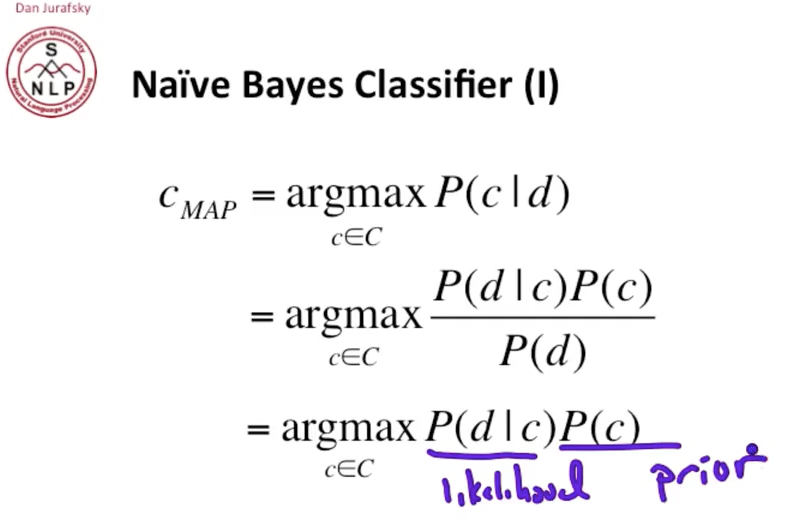
\includegraphics[width=0.5\textwidth]{multinomialNB-clsfy}
\caption[Clasificador Naïve Bayes]{Clasificador Naïve Bayes \citep{Jurafsky2015}}
\label{fig:multinomialNB-clsfy}
\end{figure}

Durante la fase de clasificación, se calculan las probabilidades de que el documento pertenezca a cada clase, tomando como cierta la clase con mayor probabilidad.
\begin{equation}
c_\text{MAP} = \argmax_{c\in C} \mathcal{P}(c|d) 
= \argmax_{c\in C} \frac{\mathcal{P}(d|c)\mathcal{P}(c)}{\mathcal{P}(d)}
= \argmax_{c\in C} \mathcal{P}(d|c)\mathcal{P}(c)
\end{equation}

El documento $d$, lo representamos por su vector de características, así
\begin{equation}
c_\text{MAP} = \argmax_{c\in C} \mathcal{P}(x_1,x_2,\ldots,x_n|c)\mathcal{P}(c)
\end{equation}

Esta transformación implica que
\begin{enumerate}
\item La posición de los términos no tiene relevancia. Por tanto, sería indistinguible de cualquier otra permutación del documento o del vector de características. 
\item Las probabilidades de cada característica $x_i$ son mutuamente independientes dada una clase $c$.
\end{enumerate}

De esta manera, podemos calcular la probabilidad conjunta $\mathcal{P}(x_1,x_2,\ldots,x_n|c)$ como
\begin{equation}
\mathcal{P}(x_1,x_2,\ldots,x_n|c) = \mathcal{P}(x_1|c) \cdot \mathcal{P}(x_2|c) \cdots \mathcal{P}(x_n|c)
\end{equation}

Y finalmente
\begin{equation}
c_\text{NB} = \argmax_{c\in C} \mathcal{P}(c) \prod_{x\in X} \mathcal{P}(x|c)
\end{equation}

Lo ponemos en práctica en el siguiente ejemplo.

\begin{example}[Clasificación NB usando BOW y 2-BOW]
Dados los documentos y los vectores de características del Ejemplo~\ref{exa:ml-bow} y Ejemplo~\ref{exa:ml-2bow}, realizar ambos entrenamientos y obtener la estimación con sus probabilidades usando el clasificador NB multinomial para los siguientes documentos de test:
\begin{enumerate}
\item ``demonstrating the adage''
\item ``demonstrating the adage amuses but none of which amounts to much of a story''
\end{enumerate}
\end{example}

La solución al ejercicio la calculamos en el \autoref{lst:multinb-bow} y \autoref{lst:multinb-2bow}. El resumen de los resultados de las predicciones puede verse en la \autoref{tbl:multinb}. Como se observa, la predicción es más intensa en el modelo 2-BOW que en el BOW. Al tener mayor número de características en consideración, hay más evidencias de la posibilidad de pertenecer a una u otra clase.

\begin{table}[htbp]
\centering
\begin{tabular}{|r|S[table-format=1.6]|S[table-format=1.6]|S[table-format=1.6]|S[table-format=1.6]|}
\hline
\multirow{2}{*}{\nombrebf{Doc.}} & \multicolumn{2}{|c|}{\nombrebf{BOW}} & \multicolumn{2}{|c|}{\nombrebf{2-BOW}} \\ \hhline{~----}
  & \multicolumn{1}{|c|}{$c_1$} & \multicolumn{1}{|c|}{$c_2$} & \multicolumn{1}{|c|}{$c_1$} & \multicolumn{1}{|c|}{$c_2$} \\ \hhline{=====}
1 & 0.029215 & 0.970784 & 0.006114 & 0.993885 \\ \hline
2 & 0.999253 & 0.000746 & 0.999999 & 0.000000 \\ \hline
\end{tabular}
\caption{Predicción de clasificación en Naïve Bayes}
\label{tbl:multinb}
\end{table}

\begin{listing}[htbp]
\begin{minted}{python}
>>> from sklearn.naive_bayes import MultinomialNB 
>>> doctest1 = "demonstrating the adage".split(' ')
>>> doctest2 = "demonstrating the adage amuses but none of which amounts to much of a story".split(' ')
>>> vectest1 = [doctest1.count(feat) for feat in features]
>>> vectest2 = [doctest2.count(feat) for feat in features]
>>> print(vectest1) # vector de características del documento de prueba 1 en BOW
[0, 0, 1, 0, 0, 0, 1, 0, 0, 0, 0, 0, 0, 0, 0, 0, 0, 0, 1, 0, 0, 0]
>>> print(vectest2) # vector de características del documento de prueba 2 en BOW
[0, 1, 1, 1, 1, 1, 1, 0, 0, 0, 0, 0, 1, 1, 2, 0, 1, 0, 1, 1, 0, 1]
>>> clsfy = MultinomialNB()
>>> clsfy.fit([vec1, vec2, vec3], [2, 2, 1])
MultinomialNB(alpha=1.0, class_prior=None, fit_prior=True)
>>> print(clsfy.classes_)
[1 2]
>>> print(clsfy.predict_proba(vectest1)) # predicción de vectest1
[[ 0.02921541  0.97078459]]
>>> print(clsfy.predict_proba(vectest2)) # predicción de vectest2
[[  9.99253463e-01   7.46536777e-04]]
>>> 
\end{minted}
\caption{Predicción NB en BOW}
\label{lst:multinb-bow}
\end{listing}

\begin{listing}[htbp]
\begin{minted}{python}
>>> from nltk.util import bigrams
>>> from sklearn.naive_bayes import MultinomialNB 
>>> doctest1 = "demonstrating the adage".split(' ')
>>> doctest2 = "demonstrating the adage amuses but none of which amounts to much of a story".split(' ')
>>> bg1 = list(bigrams(doctest1)) + [(w,) for w in doctest1]
>>> bg2 = list(bigrams(doctest2)) + [(w,) for w in doctest2]
>>> vectest1 = [bg1.count(feat) for feat in features]
>>> vectest2 = [bg2.count(feat) for feat in features]
>>> print(vectest1) # vector de características del documento de prueba 1 en 2-BOW
[0, 0, 0, 0, 1, 0, 0, 0, 0, 0, 0, 0, 1, 1, 0, 0, 0, 0, 0, 0, 0, 0, 0, 0, 0, 0, 0, 0, 0, 0, 0, 0, 0, 0, 0, 0, 1, 1, 0, 0, 0, 0, 0, 0, 0]
>>> print(vectest2) # vector de características del documento de prueba 2 en 2-BOW
[0, 0, 1, 1, 1, 0, 1, 1, 1, 1, 1, 1, 1, 1, 0, 0, 0, 0, 0, 0, 0, 0, 0, 1, 1, 1, 1, 2, 1, 0, 1, 0, 0, 1, 0, 0, 1, 1, 0, 1, 1, 0, 0, 1, 1]
>>> clsfy = MultinomialNB()
>>> clsfy.fit([vec1, vec2, vec3], [2, 2, 1])
MultinomialNB(alpha=1.0, class_prior=None, fit_prior=True)
>>> print(clsfy.classes_)
[1 2]
>>> print(clsfy.predict_proba(vectest1)) # predicción de vectest1
[[ 0.00611419  0.99388581]]
>>> print(clsfy.predict_proba(vectest2)) # predicción de vectest2
[[  9.99999838e-01   1.62105831e-07]]
\end{minted}
\caption{Predicción NB en 2-BOW}
\label{lst:multinb-2bow}
\end{listing}

\subsection{Naïve Bayes Gausiano}

Este modelo es idéntico al modelo de predicción en Naïve Bayes multinomial, con la diferencia de que se puede aplicar en datos con variables continuas \citep[Naive Bayes classifier]{wikipedia-es}. Se asume que la variable se distribuye en una curva gausiana, entonces se calcula la media $\mu_c$ y la varianza $\sigma^2_c$ de cada característica $x_i$ en los ejemplos de cada clase $c$, y se toma como valor de verosimilitud el siguiente:
\begin{equation}
\mathcal{P}(x_i=v|c) = \frac{1}{\sqrt{2\pi\sigma^2_c}}\exp\left(-\frac{(v-\mu_c)^2}{2\sigma^2_c}\right)
\end{equation}

\subsection{Análisis de discriminante lineal y cuadrático (LDA, QDA)}

La técnica de \nombrebf{análisis del discriminante lineal}\index{discriminante!lineal} o \nombrebf{cuadrático}\index{discriminante!cuadrático} (\emph{Linear and quadratic discriminant analysis}, LDA, QDA)\index{LDA}\index{QDA} es una técnica que permite reducir el número de características que sean irrelevantes o que contribuyan poco a la diferenciación de las clases \citep[Discriminant function analysis]{wikipedia-en}.

El objetivo del algoritmo es construir una combinación lineal sobre las características que:
\begin{itemize}
\item Maximice la separación entre los centroides de las clases.
\item Minimice la separación entre los ejemplos de cada clase.
\end{itemize}

En la \autoref{fig:lda} se puede ver la función discriminante $D$ que ha calculado el algoritmo en el caso de 2 dimensiones (2 características). La recta ortogonal a ésta que pasa por el punto de intersección más alto de ambas distribuciones normales es la que sirve de separación entre las dos clases.

En la versión lineal, se asume que la covarianza en las características de cada clase es constante; mientras que en la versión cuadrática del modelo, no se tiene en cuenta esta asunción y el espacio de decisión puede ser cuadrático (\autoref{fig:lda-qda}).

\begin{figure}[htbp]
\centering
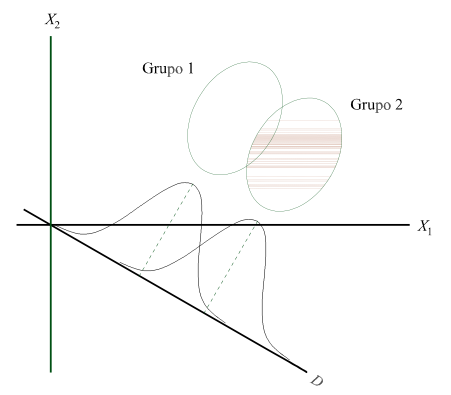
\includegraphics[width=0.6\textwidth]{lda}
\caption[Función discriminante]{Función discriminante \citep{Ruiz2001}}
\label{fig:lda}
\end{figure}

\begin{figure}[htbp]
\centering
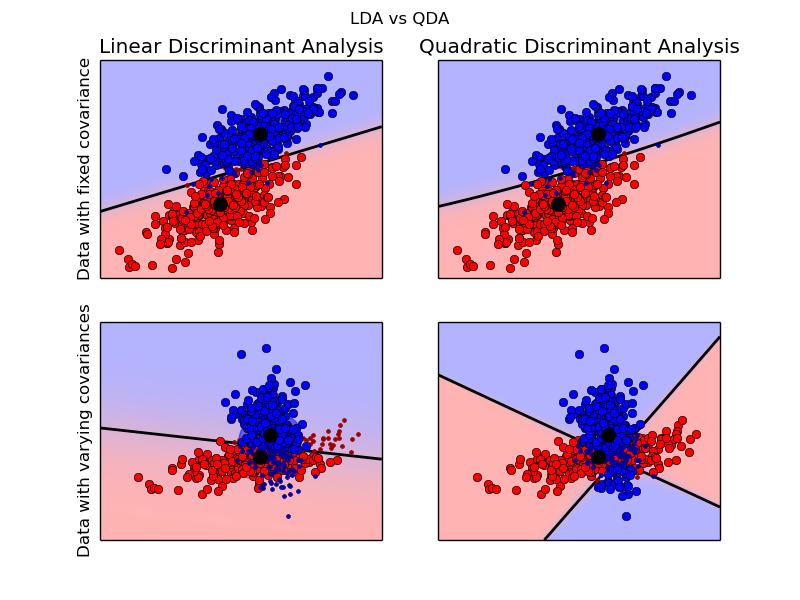
\includegraphics[width=0.7\textwidth]{plot_lda_qda_0011}
\caption[Ejemplo gráfico de discriminantes lineal y cuadrático (LDA, QDA)]{Ejemplo gráfico de discriminantes lineal y cuadrático (LDA, QDA) \citep{Pedregosa2011}}
\label{fig:lda-qda}
\end{figure}

En el \autoref{lst:lda} podemos ver un ejemplo de clasificación de este método en Scikit-Learn.

\begin{listing}[htbp]
\begin{minted}{python}
>>> import numpy as np
>>> X = np.array([[-1, -1, 0.1], [-2, -1, 0], [-3, -2, 0.3], [1, 1.1, 0.2], [2, 1, 0.7], [3, 2, 0.6]])
>>> y = np.array([1, 1, 1, 2, 2, 2])
>>> 
>>> from sklearn.lda import LDA
>>> clf = LDA()
>>> clf.fit(X, y)
LDA(n_components=None, priors=None, shrinkage=None, solver='svd',
  store_covariance=False, tol=0.0001)
>>> print(clf.classes_)
[1 2]
>>> print(clf.predict_proba([[-0.8, -1, 0.7]]))
[[ 0.99719891  0.00280109]]
>>> 
\end{minted}
\caption{Uso del clasificador de discriminante lineal (LDA)}
\label{lst:lda}
\end{listing}


\subsection{Máquinas de vectores de soporte (SVM)}

Las \nombrebf{máquinas de vectores de soporte}\index{vectores de soporte!máquinas de} (\emph{Support Vector Machines}, SVM)\index{SVM}\index{machines@\emph{machines}}\index{machines!support vector@\emph{support vector}} son algoritmos de aprendizaje supervisado que se pueden usar para clasificación, regresión y detección de valores atípicos\index{valor atípico} \emph{(outliers)}\index{outlier@\emph{outlier}} \citep{Pedregosa2011}.

Su utilidad está indicada especialmente en los siguientes casos:
\nopagebreak
\begin{itemize}
\item Cuando no se dispone de otra información a priori sobre el dominio de aplicación.
\item En espacios de dimensionalidad muy alta (cuando existe una gran cantidad de características a considerar), incluso cuando el número de dimensiones es superior al número de ejemplos de entrenamiento.
\end{itemize}

En la fase de aprendizaje, el algoritmo intenta construir un \nombrebf{hiperplano lineal}\index{hiperplano lineal} (o conjunto de hiperplanos para el caso de clasificación múltiple) que divide el espacio vectorial en dos mitades separando las clases con el mayor margen posible \emph{(maximum margin separator)}. No es necesario recordar todo el conjunto de puntos de cada clase, tan sólo los más cercanos al hiperplano (véase la \autoref{fig:svm1}).

\begin{figure}[htbp]
\centering
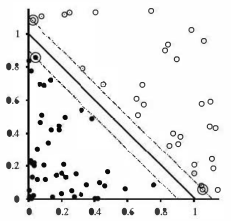
\includegraphics[width=0.4\textwidth]{svm1}
\caption[Separación mediante SVM]{Separación mediante SVM. Los vectores de soporte son los 3 puntos marcados en las fronteras de la separación, y la recta que está en el punto medio es el hiperplano (separador de margen máximo) detectado \citep{Russell2009}.}
\label{fig:svm1}
\end{figure}

Los SVMs son muy útiles para separar clases no linealmente separables en el espacio de origen. Para ello, se puede transformar el conjunto de entrenamiento añadiendo una o más dimensiones; es decir: teniendo más características en cuenta. Siempre se puede encontrar un espacio de dimensión superior en el que las clases sean linealmente separables \citep[cap. 18]{Russell2009}.

\begin{example}\label{exa:svm-circulo-separable}
Sean una serie de puntos de entrenamiento con dos características $(x_1,x_2)$, en el que los ejemplos positivos se encuentran dentro del círculo $1 = x^2 + y^2$ y los negativos fuera. En un espacio de dos dimensiones, no se puede construir una recta que separe las dos clases. Pero estableciendo la siguiente transformación
\[
\left(x_1, x_2\right) \longrightarrow \left(x_1^2, x_2^2, \sqrt{2} x_1 x_2\right)
\]
sí se puede realizar la separación con un hiperplano (un plano regular) en un espacio tridimensional (\autoref{fig:svm-circulo-separable}).
Esta función de transformación recibe el nombre de \nombrebf{kernel}\index{kernel}.
\end{example}

\begin{figure}[htbp]
\centering
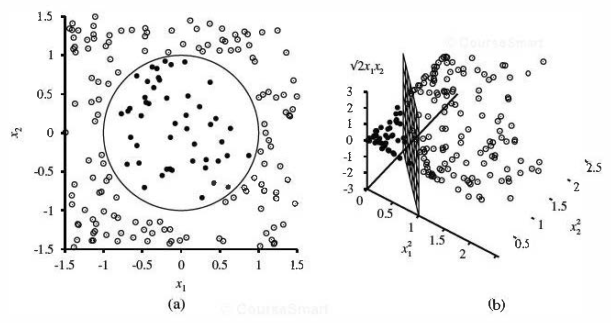
\includegraphics[width=0.85\textwidth]{svm-circulo-separable}
\caption[Sobredimensionamiento del espacio para hacer las clases linealmente separables]{Sobredimensionamiento del espacio para hacer las clases linealmente separables \citep{Russell2009}.}
\label{fig:svm-circulo-separable}
\end{figure}

El modelo trata de encontrar el vector dual de pesos $\vec{\alpha}$ realizando el producto escalar (por eso es un método muy eficiente) de los que serán los dos vectores de soporte $\vec{x_j}$ y $\vec{x_k}$ que sirvan de frontera para el separador de margen máximo, siendo $y_j, y_k \in \{-1, 1\}$ las clases de $\vec{x_j}$ y $\vec{x_k}$, respectivamente; en la ecuación \eqref{eqn:SVM}.
\begin{equation}
\argmax_\alpha \sum_j \alpha_j - \frac{1}{2} \sum_{j,k}\alpha_j \alpha_k y_j y_k (\vec{x_j} \cdot \vec{x_k})
\label{eqn:SVM}
\end{equation}

En el caso de ser necesario su transformación a un espacio de dimensión superior, se utiliza la función kernel aplicado a la pareja de ejemplos $K(\vec{x_j}, \vec{x_k})$; que sutituyendo en \eqref{eqn:SVM} queda
\begin{equation}
\argmax_\alpha \sum_j \alpha_j - \frac{1}{2} \sum_{j,k}\alpha_j \alpha_k y_j y_k (K(\vec{x_j},\vec{x_k}))
\label{eqn:SVM-kerneled}
\end{equation}

En el ejemplo~\ref{exa:svm-circulo-separable} se usó la función kernel $K(\vec{x_j},\vec{x_k})=(\vec{x_j}\cdot\vec{x_k})^2$; pero se pueden usar otras \citep{Russell2009}, como el kernel polinómico $K(\vec{x_j},\vec{x_k})=(1+\vec{x_j}\cdot\vec{x_k})^d$.
